%% For double-blind review submission, w/o CCS and ACM Reference (max submission space)
\documentclass[sigplan]{acmart}\settopmatter{printfolios=true,printccs=false,printacmref=false}
%\settopmatter{authorsperrow=2}
%% For double-blind review submission, w/ CCS and ACM Reference
%\documentclass[sigplan,review,anonymous]{acmart}\settopmatter{printfolios=true}
%% For single-blind review submission, w/o CCS and ACM Reference (max submission space)
%\documentclass[sigplan,review]{acmart}\settopmatter{printfolios=true,printccs=false,printacmref=false}
%% For single-blind review submission, w/ CCS and ACM Reference
%\documentclass[sigplan,review]{acmart}\settopmatter{printfolios=true}
%% For final camera-ready submission, w/ required CCS and ACM Reference
%\documentclass[sigplan]{acmart}\settopmatter{}


%% Conference information
%% Supplied to authors by publisher for camera-ready submission;
%% use defaults for review submission.
\acmConference[]{Project Report}{June 8, 2020}{Runtime Verification, Inc.}
\acmYear{2020}
\acmISBN{} % \acmISBN{978-x-xxxx-xxxx-x/YY/MM}
\acmDOI{} % \acmDOI{10.1145/nnnnnnn.nnnnnnn}
\startPage{1}

%% Copyright information
%% Supplied to authors (based on authors' rights management selection;
%% see authors.acm.org) by publisher for camera-ready submission;
%% use 'none' for review submission.
\setcopyright{none}
%\setcopyright{acmcopyright}
%\setcopyright{acmlicensed}
%\setcopyright{rightsretained}
%\copyrightyear{2018}           %% If different from \acmYear

%% Bibliography style
\bibliographystyle{ACM-Reference-Format}
%% Citation style
%\citestyle{acmauthoryear}  %% For author/year citations
%\citestyle{acmnumeric}     %% For numeric citations
%\setcitestyle{nosort}      %% With 'acmnumeric', to disable automatic
                            %% sorting of references within a single citation;
                            %% e.g., \cite{Smith99,Carpenter05,Baker12}
                            %% rendered as [14,5,2] rather than [2,5,14].
%\setcitesyle{nocompress}   %% With 'acmnumeric', to disable automatic
                            %% compression of sequential references within a
                            %% single citation;
                            %% e.g., \cite{Baker12,Baker14,Baker16}
                            %% rendered as [2,3,4] rather than [2-4].


%%%%%%%%%%%%%%%%%%%%%%%%%%%%%%%%%%%%%%%%%%%%%%%%%%%%%%%%%%%%%%%%%%%%%%
%% Note: Authors migrating a paper from traditional SIGPLAN
%% proceedings format to PACMPL format must update the
%% '\documentclass' and topmatter commands above; see
%% 'acmart-pacmpl-template.tex'.
%%%%%%%%%%%%%%%%%%%%%%%%%%%%%%%%%%%%%%%%%%%%%%%%%%%%%%%%%%%%%%%%%%%%%%


%% Some recommended packages.
\usepackage{booktabs}   %% For formal tables:
                        %% http://ctan.org/pkg/booktabs
\usepackage{subcaption} %% For complex figures with subfigures/subcaptions
                        %% http://ctan.org/pkg/subcaption

\usepackage{listings}
\usepackage{tikz}
\usetikzlibrary{positioning}
\usetikzlibrary{graphs}

%\usepackage{amssymb}

% colors
\definecolor{shadecolor}{gray}{1.00}
\definecolor{darkgray}{gray}{0.30}
\definecolor{violet}{rgb}{0.56, 0.0, 1.0}
\definecolor{forestgreen}{rgb}{0.13, 0.55, 0.13}

% Col language definition
\lstdefinelanguage{Coq} {
mathescape=true,						
texcl=false,
morekeywords=[1]{
  Add,
  All,
  Arguments,
  Axiom,
  Bind,
  Canonical,
  Check,
  Close,
  CoFixpoint,
  CoInductive,
  Coercion,
  Contextual,
  Corollary,
  Defined,
  Definition,
  Delimit,
  End,
  Example,
  Export,
  Fact,
  Fixpoint,
  Goal,
  Graph,
  Hint,
  Hypotheses,
  Hypothesis,
  Implicit,
  Implicits,
  Import,
  Inductive,
  Lemma,
  Let,
  Local,
  Locate,
  Ltac,
  Maximal
  Module,
  Morphism,
  Next,
  Notation,
  Obligation,
  Open,
  Parameter,
  Parameters,
  Prenex,
  Print,
  Printing,
  Program,
  Projections,
  Proof,
  Proposition,
  Qed,
  Record,
  Relation,
  Remark,
  Require,
  Reserved,
  Resolve,
  Rewrite,
  Save,
  Scope,
  Search,
  Section,
  Show,
  Strict,
  Structure,
  Tactic,
  Theorem,
  Unset,
  Variable,
  Variables,
  View,
  inside,
  outside
},
morekeywords=[2]{
  as,
  cofix,
  else,
  end,
  exists,
  exists2,
  fix,
  for,
  forall,
  fun,
  if,
%  in,
  is,
  let,
  match,
  nosimpl,
  of,
  return,
  struct,
  then,
  vfun,
  with
},
morekeywords=[3]{Type, Prop, Set, True, False},
morekeywords=[4]{
  after,
  apply,
  assert,
  auto,
  bool_congr,
  case,
  change,
  clear,
  compute,
  congr,
  cut,
  cutrewrite,
  destruct,
  elim,
  field,
  fold,
  generalize,
  have,
  heval, 
  hnf,
  induction,
  injection,
  intro,
  intros,
  intuition,
  inversion,
  left,
  loss,
  move,
  nat_congr,
  nat_norm,
  pattern,
  pose,
  refine,
  rename,
  replace,
  revert,
  rewrite,
  right,
  ring,
%  set,
  simpl,
  split,
  suff,
  suffices,
  symmetry,
  transitivity,
  trivial,
  unfold,
  unlock,
  using,
  without,
  wlog,
  autorewrite
},        
morekeywords=[5]{
  assumption,
  by,
  contradiction,
  done,
  exact,
  lia,
  gappa,
  omega,
  reflexivity,
  romega,
  solve,
  tauto,
  discriminate,
  unsat
},
morecomment=[s]{(*}{*)},
morekeywords=[6]{do, first, try, idtac, repeat},
showstringspaces=false,
morestring=[b]",
% Size of tabulations
tabsize=3,							
% Enables ASCII chars 128 to 255
extendedchars=true,  		 		
% Case sensitivity
sensitive=true, 
% Automatic breaking of long lines
breaklines=false,
% Default style fors listings
%basicstyle=\scriptsize\ttfamily,
basicstyle=\footnotesize\ttfamily,
% Position of captions is bottom
captionpos=b,							
% Full flexible columns 
columns=[l]fullflexible,
% Style for (listings') identifiers
identifierstyle={\color{black}},
% Style for declaration keywords
keywordstyle=[1]{\color{violet}},
% Style for gallina keywords
keywordstyle=[2]{\color{forestgreen}},
% Style for sorts keywords
keywordstyle=[3]{\color{forestgreen}},
% Style for tactics keywords
keywordstyle=[4]{\color{blue}},
% Style for terminators keywords
keywordstyle=[5]{\color{red}},
%Style for iterators
keywordstyle=[6]{\color{violet}},
% Style for strings
stringstyle=,
% Style for comments
commentstyle=\it\ttfamily\color{brown},
% Style for lines numbering
numberstyle=\tiny,
literate={\\/}{{$\lor~$}}1
         {/\\}{{$\land~$}}1
         {<>}{{$\neq~$}}1
         {<->}{{$\leftrightarrow~$}}1
         {:->}{{$\mapsto~$\!}}1
         {\\->}{{$\mapsto~$\!}}1
         {<--}{{$\asgn~$}}1
         {\\in}{{$\in~$}}1
         {\\notin}{{$\notin~$}}1
         {++}{{$+\!+\!~$}}1
         {->}{{$\to~$}}1
         {forall}{{$\forall~$}}1
         {exists}{{$\exists~$}}1
         {=>}{{$\Rightarrow~$}}1
         {\\~}{{$\lnot\;$}}1
%         {\\+}{{$\!\join\!~$}}1
}

\lstdefinestyle{Coq}{language=Coq}
\lstset{language=Coq}


%\lstset{%
%  literate={->}{{$\rightarrow$ }}3
%}

\begin{document}

%% Title information
\title{Verifying Gasper with Dynamic Validator Sets in Coq}         %% [Short Title] is optional;
                                        %% when present, will be used in
                                        %% header instead of Full Title.
%\titlenote{with title note}             %% \titlenote is optional;
                                        %% can be repeated if necessary;
                                        %% contents suppressed with 'anonymous'
%\subtitle{Subtitle}                     %% \subtitle is optional
%\subtitlenote{with subtitle note}       %% \subtitlenote is optional;
                                        %% can be repeated if necessary;
                                        %% contents suppressed with 'anonymous'


%% Author information
%% Contents and number of authors suppressed with 'anonymous'.
%% Each author should be introduced by \author, followed by
%% \authornote (optional), \orcid (optional), \affiliation, and
%% \email.
%% An author may have multiple affiliations and/or emails; repeat the
%% appropriate command.
%% Many elements are not rendered, but should be provided for metadata
%% extraction tools.

%% Author with single affiliation.
\author{Musab A. Alturki}
%\authornote{with author1 note}          %% \authornote is optional;
%                                       %% can be repeated if necessary
%\orcid{nnnn-nnnn-nnnn-nnnn}             %% \orcid is optional
\affiliation{
  %\position{Position1}
  %\department{Department1}              %% \department is recommended
  \institution{Runtime Verification, Inc.}            %% \institution is required
  %\streetaddress{Street1 Address1}
  %\city{City1}
  %\state{State1}
  %\postcode{Post-Code1}
  %\country{USA}                    %% \country is recommended
}
\email{musab.alturki@runtimeverification.com}          %% \email is recommended

\author{Elaine Li}
\affiliation{
  %\position{Position1}
  %\department{Department1}              %% \department is recommended
  \institution{Runtime Verification, Inc.}            %% \institution is required
  %\streetaddress{Street1 Address1}
  %\city{City1}
  %\state{State1}
  %\postcode{Post-Code1}
  %\country{USA}                    %% \country is recommended
}
\email{elaine.li@runtimeverification.com}          %% \email is recommended

%% Author with single affiliation.
\author{Daejun Park}
%\authornote{with author1 note}          %% \authornote is optional;
%                                       %% can be repeated if necessary
%\orcid{nnnn-nnnn-nnnn-nnnn}             %% \orcid is optional
\affiliation{
  %\position{Position1}
  %\department{Department1}              %% \department is recommended
  \institution{Runtime Verification, Inc.}            %% \institution is required
  %\streetaddress{Street1 Address1}
  %\city{City1}
  %\state{State1}
  %\postcode{Post-Code1}
  %\country{USA}                    %% \country is recommended
}
\email{daejun.park@runtimeverification.com}          %% \email is recommended

\author{Brandon Moore}
\affiliation{
  %\position{Position1}
  %\department{Department1}              %% \department is recommended
  \institution{Runtime Verification, Inc.}            %% \institution is required
  %\streetaddress{Street1 Address1}
  %\city{City1}
  %\state{State1}
  %\postcode{Post-Code1}
  %\country{USA}                    %% \country is recommended
}
\email{brandon.moore@runtimeverification.com}          %% \email is recommended

%% Author with single affiliation.
\author{Karl Palmskog}
%\authornote{with author1 note}          %% \authornote is optional;
%                                       %% can be repeated if necessary
%\orcid{nnnn-nnnn-nnnn-nnnn}             %% \orcid is optional
\affiliation{
  %\position{Position1}
  %\department{Department1}              %% \department is recommended
  \institution{KTH Royal Institute of Technology}            %% \institution is required
  %\streetaddress{Street1 Address1}
  %\city{City1}
  %\state{State1}
  %\postcode{Post-Code1}
  %\country{USA}                    %% \country is recommended
}
\email{palmskog@kth.se}          %% \email is recommended

%% Author with single affiliation.
\author{Lucas Pe{\~n}a}
%\authornote{with author1 note}          %% \authornote is optional;
                                        %% can be repeated if necessary
%\orcid{nnnn-nnnn-nnnn-nnnn}             %% \orcid is optional
%\affiliation{
%  %\position{Position1}
%  %\department{Department1}              %% \department is recommended
%  \institution{Runtime Verification, Inc.}            %% \institution is required
%  %\streetaddress{Street1 Address1}
%  %\city{City1}
%  %\state{State1}
%  %\postcode{Post-Code1}
%  %\country{USA}                    %% \country is recommended
%}
%\email{lucas.pena@runtimeverification.com}          %% \email is recommended
\affiliation{
  %\position{Position1}
  %\department{Department1}              %% \department is recommended
  \institution{University of Illinois at Urbana-Champaign}            %% \institution is required
  %\streetaddress{Street1 Address1}
  %\city{City1}
  %\state{State1}
  %\postcode{Post-Code1}
  %\country{USA}                    %% \country is recommended
}
\email{lpena7@illinois.edu}          %% \email is recommended

\author{Grigore Ro{\c s}u}
\affiliation{
  %\position{Position1}
  %\department{Department1}              %% \department is recommended
  \institution{Runtime Verification, Inc.}            %% \institution is required
  %\streetaddress{Street1 Address1}
  %\city{City1}
  %\state{State1}
  %\postcode{Post-Code1}
  %\country{USA}                    %% \country is recommended
}
\email{grigore.rosu@runtimeverification.com}          %% \email is recommended
\affiliation{
  %\position{Position1}
  %\department{Department1}              %% \department is recommended
  \institution{University of Illinois at Urbana-Champaign}            %% \institution is required
  %\streetaddress{Street1 Address1}
  %\city{City1}
  %\state{State1}
  %\postcode{Post-Code1}
  %\country{USA}                    %% \country is recommended
}
\email{grosu@illinois.edu}          %% \email is recommended

%\shortauthors{Palmskog, Gligoric, Pe{\~n}a, and Ro{\c s}u}

%% Abstract
%% Note: \begin{abstract}...\end{abstract} environment must come
%% before \maketitle command
\begin{abstract}
Gasper is an abstract proof-of-stake protocol layer that is implemented by the Beacon Chain protocol, the underlying protocol of the Ethereum 2.0 network. A key component of Gasper is a finality mechanism that extends the original Casper FFG protocol primarily with k-finalization. In addition to the accountable safety and plausible liveness properties, Gasper describes how the protocol generalizes to the setting of dynamic validator sets and gives a lower bound on validator stake that can provably be slashed in this setting. This report describes our effort to model and verify this finality mechanism of Gasper with dynamic validator sets using the Coq proof assistant. We outline the salient details on finality in the protocol, describe
previous verification efforts of Casper on which this work builds, and give an overview of the formal definitions and properties proved. 
The Coq source files are available at:\\
\url{github.com/runtimeverification/beacon-chain-verification/tree/master/casper/coq}
\end{abstract}


%% 2012 ACM Computing Classification System (CSS) concepts
%% Generate at 'http://dl.acm.org/ccs/ccs.cfm'.
%\begin{CCSXML}
%<ccs2012>
%<concept>
%<concept_id>10011007.10011006.10011008</concept_id>
%<concept_desc>Software and its engineering~General programming languages</concept_desc>
%<concept_significance>500</concept_significance>
%</concept>
%<concept>
%<concept_id>10003456.10003457.10003521.10003525</concept_id>
%<concept_desc>Social and professional topics~History of programming languages</concept_desc>
%<concept_significance>300</concept_significance>
%</concept>
%</ccs2012>
%\end{CCSXML}

%\ccsdesc[500]{Software and its engineering~General programming languages}
%\ccsdesc[300]{Social and professional topics~History of programming languages}
%% End of generated code


%% Keywords
%% comma separated list
%\keywords{keyword1, keyword2, keyword3}  %% \keywords are mandatory in final camera-ready submission

%% \maketitle
%% Note: \maketitle command must come after title commands, author
%% commands, abstract environment, Computing Classification System
%% environment and commands, and keywords command.
\maketitle
\renewcommand{\shortauthors}{K. Palmskog, M. Gligoric, L. Pe{\~n}a, B. Moore, and G. Ro{\c s}u}

% Casper -> finality
% Beacon chain
% sentence on sharding

\section{Introduction}
\label{sec:intro}

Ethereum 2.0~\cite{Wood2014,Eth2Specs} is a major upgrade to the Ethereum platform~\cite{Wood2014} that introduces a new proof-of-stake protocol, the Beacon Chain protocol~\cite{Beacon}, with the primary goal of increasing efficiency, scalability and security of Ethereum. Participating nodes in the protocol, called validators, lock up a portion of their holdings of the underlying currency of the platform (Ether) so that they may be chosen as members of committees that propose and validate new blocks. The beacon chain protocol is built on top of important gadgets, including Casper FFG~\cite{Buterin2017} for finalizing blocks and slashing finalization violations, LMD GHOST~\cite{ButerinBHKPQRSWZ:2020} as the fork-choice rule for determining the canonical chain, a rewards/penalties system for incentivizing proper validation behavior, a mechanism for managing validators joining and exiting the network, and a form of RANDAO-based pseudo-randomization for decentralized committee selection. 

%As in any distributed consensus protocol, two fundamental properties are desirable: safety, no two blocks belonging to two different forks in the blockchain are both finalized, and liveness, block production in the blockchain is never deadlocked. 

Gasper~\cite{ButerinBHKPQRSWZ:2020} is an abstraction of the Beacon Chain protocol that focuses on finality of blocks. %It is the combination of Casper FFG and the LMD GHOST mechanisms. 
A key component of Gasper is a finality mechanism that generalizes the original Casper FFG protocol, primarily by allowing a more general form of finalization. As in other Byzantine Fault Tolerant protocols, a key underlying assumption is that a super-majority of validators (by deposited stake) are honest and are following the protocol. If a validator attempts to deviate from the protocol (either intentionally to mount an attack or unintentionally due to an implementation error) and submits conflicting votes to blocks, the validator is penalized by having some significant portion of its deposited stake slashed. The protocol defines what constitutes conflicting votes, called the slashing conditions. Gasper aims to provide a high-level and mathematically precise description of finality that can be used to state and prove these conditions and the two key properties of the protocol: accountable safety and plausible liveness:
\begin{itemize}
\item Accountable Safety: No two blocks belonging to two different forks in the blockchain are both finalized unless at least $\frac{1}{3}$ of validators (by deposit) is provably slashable.
\item Plausible Liveness: Regardless of what happened in the past, the block finalization process can never be deadlocked.
\end{itemize}

Gasper describes another generalization of Casper in which the set of validators can change over time, which is implemented by the Beacon Chain protocol. Validators may join the network (by depositing stake) or leave the network (and reclaim their staked deposit). Dynamic validator sets introduce another challenging problem: the system is now less likely to be able to provably slash the misbehaving validators since they may now misbehave and then leave the network before their deposits are actually slashed. Therefore, in addition to safety and liveness, Gasper describes a third property, the slashable bound, that gives a lower bound on the slashable stake in the system expressed in terms of validator activations and exits, which can be controlled by external policies. Finally, Gasper also handles ``probabilistic liveness''~\cite{ButerinBHKPQRSWZ:2020}, which quantifies the likelihood of finalizing a new block given certain assumptions about good validator behavior. This property, however, is outside the scope of this work.

In this work, we formalize the finality mechanism of Gasper (the latest Casper version) in the general setting of dynamic validator sets in Coq. We state and prove all three key properties of Gasper in this setting: accountable safety, plausible liveness and the slashable bound theorem, all in the same Coq model. Deductive verification with Coq of the protocol gives the greatest confidence in the correctness and completeness of arguments, ensuring that there are no unstated assumptions or invalid deduction steps. The formalization also feeds back into the description of the protocol making it more precise and complete. We describe our effort in this report and explain how the formalization was developed and in what ways this formalization helped improve the original statements and arguments in the Gasper paper~\cite{ButerinBHKPQRSWZ:2020}.

This work builds on our previous initial attempt at mechanizing the original Casper FFG protocol~\cite{PalmskogPGPR:2019,PalmskogPGPMR:2018,CasperProofs}, which in turn benefited greatly from earlier work by others~\cite{pos,Pirlea2018,Toychain}. The four major improvements/additions compared with our previous work are:
\begin{enumerate}
\item Unifying the two models previously developed for safety and liveness into one model against which all properties are stated and proved. As a side product of this unification, some facts that were only assumed in our earlier models are now provable results, while other assumptions had to be slightly modified.
\item Modeling the more general k-finalization of Gasper, in which the finalization chain can be of any length $k \geq 1$. 
\item Modeling the more general setting of dynamic validator sets, resulting in updated proofs of accountable safety and plausible liveness.
\item Modeling validator set weights and proving the slashable bound theorem.
\end{enumerate}

The report is organized as follows. In the next section, we give some background on relevant work on formalizing Casper in Coq. This is followed in Section 3 by a description of our modeling approach. Section 4 explains the accountable safety formalization and proof. Then, in Section 5, we describe the Plausible Liveness property. We then explain in Section 6 how the slashable bound theorem is specified and proved. Section 7 discusses the results as they compare with Gasper's description. Section 8 concludes the report. 


\section{Background}
\label{sec:background}
This section explains blockchain and Casper terminology, provides pertinent Coq
background, and describes the previous formalization and verification efforts we
build upon.

% We build directly on two previous modeling and verification efforts: verified
% abstract models of various versions of Casper in Isabelle/HOL by
% Hirai~\cite{pos}, and a model in Coq of a distributed blockchain system called
% Toychain by P{\^{\i}}rlea and Sergey~\cite{Pirlea2018}. We give a brief overview
% of the Casper finality system and each of these two pillars.

\subsection{Blockchain and Casper Terminology}

Abstractly, the global state in a blockchain system is a \emph{block forest},
with a unique genesis block that is the root of a special \emph{block tree}.
Trees not rooted in the genesis block may be possible but are typically
disregarded.
As new blocks arrive to the system, nodes in the system continually establish
consensus on a canonical blockchain defined by one of the leaves in the special
block tree.
New blocks are minted through a \emph{proposal} mechanism, which could be an
underlying blockchain using proof-of-work~\cite{Nakamoto2008} or
proof-of-stake~\cite{proof-of-stake} to regulate block creation.
Participating nodes use a local \emph{fork choice rule} to decide where
to construct a new block onto the current block tree.
Due to, e.g., delays or adversarial behavior, there may be competing leaf blocks
of similar tree height, defining different blockchain \emph{forks}.

Casper, the finalization tool in Gasper, overlays a blockchain system, and intuitively works by engaging a group
of autonomous \emph{validators} who attest to, by broadcasting votes, that
certain blocks in the special tree belong to the designated canonical
blockchain.
To participate, validators must demonstrate that they have a stake in the
blockchain system by locking up a \emph{deposit} of the blockchain's cryptocurrency.
The deposit will be \emph{slashed} if the validator is verifiably reported by
other validators to be behaving adversarially. Moreover, validators may be allowed to join and leave the network and thus the set of active validators may change over time during the execution of the protocol.

For verification, we focus on the three main properties of Gasper that were proved
informally in~\cite{ButerinBHKPQRSWZ:2020} (i.e. without using a mechanical proof
assistant): accountable safety, plausible liveness and the slashable bound theorem, assuming dynamic validator sets.
Accountable safety intuitively states that conflicting blocks in different block
tree forks cannot both be finalized if more than $\frac{2}{3}$ of validators (by
deposit) behave honestly.
Plausible liveness states that regardless of what has happened before, it is
always possible to continue to finalize blocks when more than $\frac{2}{3}$ of
validators follow the protocol. Finally, the slashable bound theorem expresses a lower bound on how much stake is provably slashable (when safety is violated) in terms of activation and exit parameters that are controllable using external policies.

\subsection{Casper Formalizations}

Yoichi Hirai formalized and verified several earlier variants of Casper in the
Isabelle/HOL proof assistant~\cite{pos}.
These formalizations are highly abstract, in the sense that they ignore most
details of the structure of hashes, blocks, and validators.
For example, the requirements on the fractions of honest validators is captured,
via Isabelle's locale mechanism~\cite{Ballarin2014}, by postulating abstract
types $'q_1$ and $'q_2$ to represent collections of sets of validators of
at least $\frac{2}{3}$ weight and sets of validators of at least $\frac{1}{3}$ weight
respectively.
Instead of any numerical details, the Isabelle formalization just assumes the
key intersection property, that any two set of validators each of at least
$\frac{2}{3}$ have a common subset of weight at least $\frac{1}{3}$.
This is how that property was expressed in Isabelle:
$$\bigwedge q_1\, q_2\, .\, \exists\, q_3\, .\, \forall\, v\, .\, v \in_2 q_3 \rightarrow v \in_1 q_1 \land v \in_1 q_2$$
% assumes "\<And> q1 q2 . \<exists> q3 . \<forall> n . n \<in>\<^sub>2 q3 \<longrightarrow> n \<in>\<^sub>1 q1 \<and> n \<in>\<^sub>1 q2"
Here, $\bigwedge$ is universal quantification,
the subscripted operator $v \in_1 q$ means that validator $v$ is a member of a
set $q$ which belongs to the type $'q_1$ that represents sets of weight at least
$\frac{2}{3}$,
and the subscripted operator $v \in_2 q$ means that validator $v$ is a member of a set $q$ which belongs to the type $'q_2$ that represents sets of weight at least $\frac{1}{3}$.
In this proposition $q_1$ and $q_2$ have type $'q_1$ and $q_3$ has type $q_2$.
This use of numbered ``q''s as both types and variables is confusing,
but exactly follows the Isabelle definition.
While accountable safety is verified for the most recent Casper, plausible
liveness is only proven for an earlier variant with different inter-validator
messages.
Moreover, these proofs were developed in an older version of Isabelle and
already the proof of accountable safety cannot be checked with Isabelle2017.

In earlier work~\cite{PalmskogPGPR:2019,PalmskogPGPMR:2018,CasperProofs}, we developed models in Coq of Casper based on Hirai's formalization. The models enabled mechanizing accountable safety and plausible liveness proofs of the then-updated Casper, assuming a fixed validator set. The work we present here in this report builds on our earlier developments and extends them in several ways as explained in Section \ref{sec:intro}.

\subsection{Mathematical Components and Toychain}
We employ several existing Coq libraries which already formalized
the majority of the mathematics we need to define and reason about Casper.
Mathematical Components~\cite{MathComp} is a Coq library based on packaging
mathematical structures and results in the form of Coq \emph{canonical
  structures}, which can be reused and specialized when
required~\cite{Garillot2009}.
The library was used by Gonthier~et~al.\ to capture finite group theory and
prove fundamental results in abstract algebra~\cite{Gonthier2013}.
In addition to structures from abstract algebra, the library also contains
encodings of and results about many standard data structures, such as numbers,
lists, and finite sets.

Toychain~\cite{Pirlea2018,Toychain} is a general formalization of blockchain
systems in Coq using the Mathematical Components library.
It defines blocks, forks, and distributed node state, but abstracts from
specific block proposal mechanisms and procedures to let nodes decide between
forks.
Toychain represents a block tree as a finite map from hashes to blocks.
Toychain describes the behavior of a blockchain system as a relation between
global states, and establishes that absent adversarial interference, the
canonical chain becomes known to all nodes in the steady state.
For example, the Toychain global state is represented as a Coq record
\begin{lstlisting}[language=Coq]
Record World := mkW { localState : StateMap;
 inFlightMsgs : seq Packet; consumedMsgs : seq Packet; }.
\end{lstlisting}
where \lstinline{localState} maps node names to their current block tree and
other local data.
We have extended and revised Toychain in collaboration with its authors to
support capturing full realistic blockchain system specifications such as that
for Bitcoin~\cite{Bitoychain}.
Our model of Casper incorporates definitions and lemmas from this extended
version of Toychain.

\section{Modeling and Verification Approach}
\label{sec:approach}
%This section outlines our approach to modeling and verifying Casper in Coq.

As highlighted above, our approach is based on a translation of Hirai's Casper definitions and theorems~\cite{pos} from
Isabelle/HOL to Coq, and relating these definitions with key
definitions from Toychain. While developing the model and the proofs, we have strived to stay close to the definitions and arguments in the Gasper paper~\cite{ButerinBHKPQRSWZ:2020} as much as possible, which helps readability of the model, and makes it easier to verify correctness of the arguments and identify any missing assumptions or reasoning steps. Naturally, the model is much more rigorous and there are aspects of the model that are necessarily different. We highlight these aspects of the model later in Section~\ref{sec:discussion}.
%At the same time, we leveraged the Toychain definitions and results to capture
%the behavior of nodes as found in the Casper-based beacon chain for
%Ethereum~\cite{Beacon}.

%Unlike 
%For tractability, we focused on translating and adapting Hirai's formal models
%with a \emph{static} validator set, which are simpler (but less realistic) than
%the corresponding models with churn among validators.

We used concepts from the Mathematical Components library to simplify forming and reasoning about finite sets, finite maps and natural numbers and expressions (see~\cite{MathComp}). Since the formal model for establishing safety by Hirai mostly uses first-order reasoning, we were able to successfully leverage the CoqHammer extension~\cite{Czajka2018,CoqHammer} to perform safety proofs in Coq that closely followed Isabelle/HOL proofs. The project's Github repository at \url{github.com/runtimeverification/beacon-chain-verification/tree/master/casper/coq} lists the project's dependencies needed to check the proofs.

Below, we highlight the main components of the model and how they are specified in Coq.

\subsection{Validators and Weights}
\label{sec:validators}

Validators are participating nodes in the network that contribute to the protocol by validating blocks, casting votes attesting to blocks and proposing new blocks. Validators are identified by fixed-size keys so we represent validators as members of a \emph{finite type}
(having a finite number of members that can be enumerated), written
\lstinline{Validator : finType}.

For a node to become a validator, it needs to have an amount of currency (Ether) locked up as its stake in the network. We represent this fact by an abstractly declared finite map (a function whose domain is a finite type) that gives the stake amount of a validator \lstinline|stake : {fmap Validator -> nat}|. Every validator must have a stake in the system (although the stake may in principle reach zero due to slashing). Therefore, we add the assumption that the stake map is total:
\begin{lstlisting}[language=Coq]
Axiom st_fun : forall v : Validator, v \in stake.
\end{lstlisting}

Moreover, we will need to reason about the combined deposits, or \textit{weights}, of validator sets, defined as the total stake amount of all validators in a set:
\begin{lstlisting}[language=Coq]
Definition wt (s:{set Validator}) : nat := 
  \sum_(v in s) stake.[st_fun v].
\end{lstlisting}
Given a set of validators \lstinline|s|, the function \lstinline|wt| computes the weight of \lstinline|s| as the sum of stake amounts of all validators in that set. The expression \lstinline|stake.[st_fun v]| is the stake for validator \lstinline|v| (which we know is well-defined since \lstinline|stake| is assumed total --- the term \lstinline|st_fun v| is a proof that \lstinline|v| is in the domain of \lstinline|stake|). 

Several important properties of \lstinline|wt| follow from its definition and basic set-theoretic laws. For example, the weight function is monotonic:
\begin{lstlisting}[language=Coq]
Lemma wt_inc_leq (s1 s2:{set Validator}):
  s1 \subset s2 -> wt s1 <= wt s2.
\end{lstlisting}
Another example is that the weight of two disjoint validator sets is exactly the sum of their weights (the symbol \lstinline{:|:} denotes set union):
\begin{lstlisting}[language=Coq]
Lemma wt_join_disjoint (s1 s2:{set Validator}):
  [disjoint s1 & s2] -> wt (s1 :|: s2) = wt s1 + wt s2.
\end{lstlisting}
These properties and several others along with their proofs can be found in \lstinline|Weights.v| in the project's repository.

\subsection{Block Forests}

The finality mechanism of Gasper (and Casper in particular) operates on epoch boundary blocks, also known as \textit{checkpoint blocks}. We therefore consider only checkpoint blocks in the model, and refer to them simply as blocks. A block is identified by a (fixed-width) hash value, so we assume a finite type of block hashes \lstinline|Hash : finType| (with member \lstinline{genesis} representing the Genesis block). To abstract a block forest, we assume a binary parent relationship on block hashes \lstinline|hash_parent : rel Hash|, for which we use the notation \lstinline|h1 <~ h2| to mean that \lstinline|h1| is a (the) parent of \lstinline|h2|, and having the following two properties:s 
\begin{enumerate}
\item A block cannot be the parent of itself:
\begin{lstlisting}[language=Coq]
Axiom hash_parent_irreflexive:
  forall h1 h2, h1 <~ h2 -> h1 <> h2.
\end{lstlisting}
\item A block can have at most one parent block:
\begin{lstlisting}[language=Coq]
Axiom hash_at_most_one_parent :
  forall h1 h2 h3, h2 <~ h1 -> h3 <~ h1 -> h2 = h3.
\end{lstlisting}
\end{enumerate}

We also define the ``ancestor'' binary relation \lstinline|<~*| as the reflexive-transitive closure of \lstinline|<~|, using the closure operation \lstinline|connect|:
\begin{lstlisting}[language=Coq]
Definition hash_ancestor h1 h2 := connect hash_parent h1 h2.
\end{lstlisting}
The notion of block ancestry is fundamental to the protocol as it enables specifying conflicting blocks, which are blocks that are not related by the ancestry relation. Several properties of the ancestry relation follow from those of the closure operation \lstinline|connect|, such as reflexivity (every block is an ancestor of itself) and concatenation (an ancestor of an ancestor is also an ancestor) among others. One basic property with special significance in the accountable safety proof is that a conflicting block cannot belong to the ancestry of that block:  
\begin{lstlisting}[language=Coq]
Lemma hash_ancestor_conflict:
  forall h1 h2 p, h1 <~* h2 -> p </~* h2 -> p </~* h1.
\end{lstlisting}
The notation \lstinline|</~*| expands to the negation of the ancestry relation \lstinline|<~*|.

Finally, we give an inductive definition of ancestry that makes the exact number of steps explicit:
\begin{lstlisting}[language=Coq]
Inductive nth_ancestor : nat -> Hash -> Hash -> Prop :=
| nth_ancestor_0 : forall h1, nth_ancestor 0 h1 h1
| nth_ancestor_nth : forall n h1 h2 h3,
    nth_ancestor n h1 h2 -> h2 <~ h3 ->
    nth_ancestor n.+1 h1 h3.
\end{lstlisting}
We show that the two definitions are compatible in the sense that they both capture the same notion of ancestry. The additional piece of information provided by \lstinline|nth_ancestor| will be useful when defining justification and finalization.

\subsection{The Global State}

Given our definitions of validators and the block forest, we define the global state as the set of votes cast by validators. Similarly to how votes are defined in Casper, we model a vote by a quintiple:
\begin{lstlisting}[language=Coq]
Definition Vote := (Validator * Hash * Hash * nat * nat)%type.
\end{lstlisting}
Each vote \lstinline|(v, s, t, s_h, t_h)| is signed by a particular validator (attester) \lstinline|v|, and names the source and target blocks (\lstinline|s| and \lstinline|t| respectively) and their attestation heights (\lstinline|s_h| and \lstinline|t_h| respectively).

The global state is defined by the finite set of votes cast:
\begin{lstlisting}[language=Coq]
Definition State := {fset Vote}.
\end{lstlisting}
Whether a vote has been cast or not can be determined by a boolean membership predicate:
\begin{lstlisting}[language=Coq]
Definition vote_msg (st:State) v s t s_h t_h : bool := 
  (v,s,t,s_h,t_h) \in st .
\end{lstlisting}

\subsection{Slashing Violations}

\begin{figure}
\textsc{An individual validator $v$ must not publish two distinct votes},
\[\langle v,s_1,t_1,h(s_1),h(t_1)\rangle \qquad \textsc{and} \qquad \langle v,s_2,t_2,h(s_2),h(t_2) \rangle,\]
\textsc{such that either}:
\begin{description}
\item[\phantom{I}I.] $h(t_1) = h(t_2).\quad$
  Equivalently, a validator must not publish two distinct votes for the same
  target height.
\item[II.] $h(s_1)<h(s_2)<h(t_2)<h(t_1).$
  Equivalently, a validator must not vote within the span of its other votes.
\end{description}
\caption{Slashing Conditions of Casper}\label{fig:slashing-conditions}
\end{figure}
With votes defined we can then define the two slashing conditions of Casper (shown
in Figure~\ref{fig:slashing-conditions}) in terms of two kinds of conflicting voting behaviors: double-voting and surround-voting.
Double-voting occurs if validator \lstinline{v} has voted for two different target blocks \lstinline{t1} and \lstinline{t2} both at height \lstinline{t_h}.
\begin{lstlisting}
Definition slashed_double_vote st v :=
  exists t1 t2, t1 <> t2 /\ exists s1 s1_h s2 s2_h t_h,
    vote_msg st v s1 t1 s1_h t_h 
    /\ vote_msg st v s2 t2 s2_h t_h.
\end{lstlisting}
Surround-voting happens if validator \lstinline{v} has made two votes so the
source height \lstinline{s1_h} and target height \lstinline{t1_h} of one vote strictly
surround the source height \lstinline{s2_h} to target height \lstinline{t2_h}
range of the other vote. 
\begin{lstlisting}
Definition slashed_surround_vote st v :=
  exists s1 t1 s1_h t1_h,
  exists s2 t2 s2_h t2_h,
    vote_msg st v s1 t1 s1_h t1_h /\
     vote_msg st v s2 t2 s2_h t2_h /\
     s2_h > s1_h /\ t2_h < t1_h.
\end{lstlisting}
We now define a proposition saying a validator is slashed in a given global state.
\begin{lstlisting}
Definition slashed st v : Prop :=
 slashed_double_vote st v \/ slashed_surround_vote st v.
\end{lstlisting}
A validator is slashed if it has either double- or surround-voted.

\subsection{Quorums}
\label{sec:quorums}

As is typical in Byzantine fault tolerant protocols, Gasper assumes that the supermajority of validators are honest. A supermajority is defined as a subset of validators whose weight is at least $\frac{2}{3}$ of the total stake. Moreover, proofs of safety and liveness generally show that an attack cannot succeed without a set of attacking validators of at least $\frac{1}{3}$ of the total stake being slashed for it. As we intend to model dynamic validator sets where the active set of validators may change across different blocks, these bounds on weights can only be defined in relation to the current set of active validators. 

Therefore, we first declare an abstract (finite) map vset : \lstinline|{fmap Hash -> {set Validator}}| that gives the active validator set for a block. Every block has a set of active validators, so we declare the map total:
\begin{lstlisting}
Axiom vs_fun : forall h : Hash, h \in vset.
\end{lstlisting}

Now the $\frac{2}{3}$ lower bound on weights of validator sets (quorums) can be specified as a predicate parametric to blocks:
\begin{lstlisting}
Definition quorum_2 (vs : {set Validator}) (b : Hash) : bool :=
  (vs \subset vset.[vs_fun b]) && 
  (wt vs >= two_third (wt vset.[vs_fun b])).
\end{lstlisting}
For a block \lstinline|b|, a validator set \lstinline|vs| is a \lstinline|quorum_2| set if it satisfies two conditions: (1) all validators in \lstinline|vs| appear in the active validator set of the block \lstinline|b|, and (2) the weight of the set \lstinline|vs| is at least $\frac{2}{3}$ of the total weight of all active validators of \lstinline|b|. 
%The \lstinline|quorum_2| predicate is similarly defined, but with the bound $\frac{2}{3}$ 
(note that the constant \lstinline|two_third| is merely used for convenience of typing with natural numbers). 

The predicate \lstinline|quorum_2| abstracts the powerset of sets of validators with weight at least $\frac{2}{3}$ of the total for a given block. For example, justifying a link from a source block to a target block requires receiving votes from all validators in a supermajority set (with respect to the target block), i.e. a subset of validators satisfying \lstinline|quorum_2| for the target block.

Given these definitions, we can now specify what it means for a quorum to be slashed using abstract membership constraints: 
\begin{lstlisting}[language=Coq]
Definition q_intersection_slashed st :=
  exists (bL bR: Hash) (vL vR: {set Validator}),
    vL \subset vset.[vs_fun bL] /\ 
    vR \subset vset.[vs_fun bR] /\
    quorum_2 vL bL /\ 
    quorum_2 vR bR /\
    forall v, v \in vL -> v \in vR -> slashed st v.
\end{lstlisting}
The proposition \lstinline|q_intersection_slashed| states that slashing a quorum means the existence of two supermajority quorums \lstinline|vL| and \lstinline|vR| with respect to some blocks \lstinline|bL| and \lstinline|bR| respectively whose intersection is slashed. Note that unlike Hirai's abstract formulations of Casper~\cite{pos} where the intersection is guaranteed to be of weight at least $\frac{1}{3}$ of the total stake, the formulation in Gasper is more general since the validator sets are dynamic and the intersection is no longer guaranteed to respect this bound (more on this in Section~\ref{sec:bound}).
 
\subsection{Justification}

A supermajority link from a source block to a target block is formed when a supermajority quorum of validators (with respect to the target block) vote for this pair of blocks. We capture this intuition by first defining the set of validators attesting for a given pair of blocks (using set comprehension notation):
\begin{lstlisting}
Definition link_supporters st s t s_h t_h : {set Validator} :=
  [set v | vote_msg st v s t s_h t_h ].
\end{lstlisting}
Now we can define a supermajority link predicate as follows:
\begin{lstlisting}
Definition supermajority_link (st:State) s t s_h t_h : bool :=
  quorum_2 (link_supporters st s t s_h t_h) t.
\end{lstlisting}
We have, in the current state, a supermajority link from block \lstinline|s| to \lstinline|t| with justification heights \lstinline|s_h| and \lstinline|t_h| respectively if and only if the set of validators voting for this link is a supermajority quorum (relative to the active validator set of the target block \lstinline|t|).

Note that a supermajority link as defined above does not yet capture proper justification links in Gasper, which must be valid forward links in the block forest with the target block being a descendant block of the source at the appropriate heights:
\begin{lstlisting}
Definition justification_link (st:State) s t s_h t_h : Prop :=
  t_h > s_h /\
  nth_ancestor (t_h - s_h) s t /\
  supermajority_link st s t s_h t_h.
\end{lstlisting}
The conjuncts respectively require that the justification height of the target block \lstinline{t_h} is strictly greater than that of the source, that the source block \lstinline{s} is actually the ancestor the appropriate number of levels above the target block \lstinline{t}, and that a supermajority quorum of validators have voted for this link in the state.

This allows us to define justified blocks inductively in terms of a path from the genesis block all the way to that block:
\begin{lstlisting}
Inductive justified (st:State) : Hash -> nat -> Prop :=
| justified_genesis : justified st genesis 0
| justified_link : forall s s_h t t_h,
    justified st s s_h ->
    justification_link st s t s_h t_h ->
    justified st t t_h.
\end{lstlisting}
The genesis block is always justified at height 0. A non-genesis block is justified if there exists a proper justification link to the block from an ancestor block that is already justified.  

\subsection{Finalization}

A justified block is finalized if there exists an immediate descendant (child) block that is also justified by a supermajority link to it. This is the original definition of finalization in Casper~\cite{Buterin2017}, which is captured by the following definition:
\begin{lstlisting}
Definition finalized st b b_h :=
  justified st b b_h /\
  exists c, (b <~ c /\ supermajority_link st b c b_h b_h.+1).
\end{lstlisting}

%[add diagram for k-finalization]

Gasper~\cite{ButerinBHKPQRSWZ:2020} generalizes finalization to k-finalization: a k-finalized block is a justified block that has a k-descendent who is also justified by a supermajority link to the block, and all blocks to the descendent are also justified. We formalize this as follows:
\begin{lstlisting}
Definition k_finalized st b b_h k :=
  k >= 1 /\ 
  exists ls, size ls = k.+1 /\
        head b ls = b /\
        (forall n, n <= k ->
              justified st (nth b ls n) (b_h+n) /\
              nth_ancestor n b (nth b ls n)
        ) /\
        supermajority_link st b (last b ls) b_h (b_h+k). 
\end{lstlisting}
The chain \lstinline|ls|, which is of length \lstinline|k + 1|, has the k-finalized block \lstinline|b| as its head. Each block in the chain is justified, with the last block (the k-descendent of \lstinline|b|) justified by a supermajority link from \lstinline|b|. %Figure~\ref{} (borrowed from~\cite{}) illustrates the definition. 

Note that $\mathtt{k} \geq 1$. When \lstinline|k| is 1, the two notions of finalization and k-finalization  coincide:
\begin{lstlisting}
Lemma finalized_means_one_finalized : forall st b b_h,
  finalized st b b_h <-> k_finalized st b b_h 1. 
\end{lstlisting}

\section{Accountable Safety}
\label{sec:safety}
This section describes the Coq formalization and verification of
Casper's \emph{accountable safety} property.
A major part of the Gasper (Casper) design is ensuring that an attack cannot
finalize blocks on both sides of a fork in the chain without the
attacker losing a significant amount of money by having their validator deposits slashed.
This is formalized as the accountable safety theorem. In the fixed validator sets setting, the theorem says that if two
blocks are finalized and neither is an ancestor of the other, then validators
having at least $\frac{1}{3}$ of the total stake must have violated the slashing
conditions~\cite{Buterin2017}. In the more general setting where validators are allowed to join and leave the network, the lower bound on the deposits that can be slashed is dependent on how much validator churn is allowed, which can be controlled by externally specified validator activation and exit policies~\cite{ButerinBHKPQRSWZ:2020}. 
Note that the difference between slashing violations and actually losing funds is
addressed and handled with other countermeasures in the protocol~\cite{Buterin2017,Beacon}.

We model the dynamic validator setting, of which the fixed validator sets setup can be obtained as a special case. We also capture Gasper's generalized accountable safety theorem in which each of the two conflicting blocks can be k-finalized for potentially two distinct values of k.

Building on the definitions of validator quorums and justification described above,
we define a k-finalization fork in a state as two conflicting k-finalized blocks (hashes):
\begin{lstlisting}[language=Coq]
Definition k_finalization_fork st k1 k2 :=
  exists b1 b1_h b2 b2_h,
    k_finalized st b1 b1_h k1 /\
    k_finalized st b2 b2_h k2 /\
    b2 </~* b1 /\ b1 </~* b2.
\end{lstlisting}
Note that the blocks are finalized at depths \lstinline|k1| and \lstinline|k2|, which may be different. Forking with same-depth finalization or with finalization at depth exactly 1 are all instances of this definition.

With \lstinline{q_intersection_slashed st} (defined in Section~\ref{sec:quorums}) capturing that a quorum of validators is slashed in state \lstinline{st} due to a violation of the slashing conditions in Figure~\ref{fig:slashing-conditions}, we define and prove accountable safety:
\begin{lstlisting}[language=Coq]
Theorem k_accountable_safety : forall st k1 k2, 
  k_finalization_fork st k1 k2 -> q_intersection_slashed st.
\end{lstlisting}
The proof roughly follows the informal arguments~\cite{ButerinBHKPQRSWZ:2020}:
\begin{enumerate}
\item If the two finalized blocks \lstinline{b1} and \lstinline{b2} were at the same height, then the validator sets corresponding to these blocks have a common quorum of validators who violated slashing condition I (double-voting for two different target blocks with the same height).
\item Otherwise, consider the path of justified links which justifies the higher finalized block (say that the higher finalized block is b2 --- the other case is symmetrical). If any justified block along this path has the same height as the other justified block \lstinline{b1} or any of its justified descendants along its k1-finalization chain, then we again have a set of validators violating slashing condition I.
\item Otherwise, find the justified link along that path with a source lower than the other justified block \lstinline{b1} and a target
higher than any of its descendants belonging to its k1-finalization chain. Taking this link along with the justified link between the k1-finalized block \lstinline{b1} and its k1-descendent, we have a set of validators violating slashing condition II.
\end{enumerate}

The mechanization in Coq structures the proofs so that each of three main cases above is proved as a separate result. Note that the third case above uses induction to traverse the path of justification links in the argument. In all cases, the proofs find exactly the pair of blocks whose validator sets have an intersection that is slashed for violating the conditions, as required to conclude \lstinline|q_intersection_slashed|.   


% The final step is analysis of two cases. In the first case, the validators
% of the two finalized blocks are distinct:
% \begin{lstlisting}[language=Coq]
% Lemma case_1 : forall s q1 q2 h1 v1 x h2 v2 xa,
%  finalized s q1 h1 v1 x -> finalized s q2 h2 v2 xa ->
%   ~ hash_ancestor h2 h1 -> h1 <> h2 -> v1 > v2 ->
%   quorum_slashed s.
% \end{lstlisting}
% In the second case, they are one and the same:
% \begin{lstlisting}[language=Coq]
% Lemma case_2 : forall s q1 h1 v1 x q2 h2 xa,
%  finalized s q1 h1 v1 x -> finalized s q2 h2 v1 xa ->
%  h1 <> h2 -> quorum_slashed s.
% \end{lstlisting}

%The key lemma 
%  finalized s q1 h1 v1 c1 ->
%  finalized s q2 h2 v2 c2 ->
%  h2 </~* h1 ->
%  h1 </~* h2 ->
%  h1 <> h2 ->
%  quorum_slashed s.

%Then the safety property is stated as saying that a
%fork can only exist in a state if some \lstinline{quorum_2}
%set of validators has been slashed:

%A block defined by the hash \lstinline{h} is justified
%at a distance \lstinline{d} from the genesis block if
%there is 
%
%%justified s parent pre ->
%%justified_link s q parent pre h now ->
%
%\begin{lstlisting}[language=Coq]
%Definition finalized s q h v c := hash_parent h c /\
% justified s h v /\ justified_link s q h v c v.+1.
%\end{lstlisting}

%\begin{lstlisting}[language=Coq]
%fork s ->
%\end{lstlisting}
%Intuitively, this property states that a fork cannot arise unless
%at least $\frac{1}{3}$ weight of validators misbehaved, and
%that if a fork does happen then at least $\frac{1}{3}$ of the
%malicious validators had their deposits slashed.
%The proof follows the informal argument~\cite{Buterin2017}.

\section{Plausible Liveness}
\label{sec:liveness}
The liveness goal for Casper is that as long as a $\frac{2}{3}$ quorum of validators (by weight) always exists and 
is following the protocol and block proposals continue, then further checkpoints
can continue to be finalized regardless of the behavior of the rest of possibly misbehaving validators, without needing any of the honest validators to violate a
slashing condition and sacrifice their deposit to allow the chain to live.

Our Coq proof is based on the argument given in~\cite{Buterin2017,ButerinBHKPQRSWZ:2020}, and also
Yoichi Hirai's Isabelle/HOL proof of plausible liveness for an older variant
of the Casper protocol~\cite{pos}. In our mechanization, we state and prove liveness in terms of the hash and height of the most recent previously-finalized block (which we prove always exists). The proof uses the same model of checkpoint blocks described in Section~\ref{sec:approach} and builds on the accountable
safety result described in Section~\ref{sec:safety} above. Therefore, compared with previous mechanizations efforts, our mechanization in Coq proves Gasper's plausible liveness property in a more general setting with dynamic validators and a generalized finalization definition.

%%Besides the parameterization over the epoch start block,
%%we do not actually consider the history of any past epochs.
%%In particular, we assume that the well-behaved nodes have not made any
%%votes with sources outside the current epoch.
%%We could work without that assumption, but we would need to repeat
%%part of the accountable safety proof to argue that an unslashed
%%validator's votes from past epochs cannot prevent them from
%%safely making the votes chosen in out proof.

\subsection{Proof Strategy and Assumptions}
To formalize a statement of plausible liveness, we 
abstract away from any implementation details of ``following the protocol'',
and simply require that our $\frac{2}{3}$ good validators have not made certain
sorts of bad votes.
For the conclusion we also ignore the details of how validators decide to make
votes, and simply show that there is some set of votes which the good validators
could make that would finalize a further block and not violate slashing conditions.

In Hirai's proof for the previous Casper design it was sufficient to simply require
that the good validators were unslashed.
The current Casper design intentionally removed any slashing conditions that required
knowing the state of the chain when the votes were made.
We found that \emph{one of these conditions was essential to the proof}, so our definition
of good behavior for the current Casper protocol requires that a validator has not
made votes with unjustified sources or votes that would represent invalid backward justification links, in addition to requiring that a good validator
had not been slashed.

Therefore, we define the property that, for any block, a super-majority-quorum validator makes only good votes:
\begin{lstlisting}
Definition good_votes (st : State) :=
  forall b q2, quorum_2 q2 b ->
    forall v, v \in q2 ->
    justified_source_votes st v /\ forward_link_votes st v.
\end{lstlisting}
The proposition \lstinline|justified_source_votes| holds when all votes cast by validator \lstinline|v| in state \lstinline|st| have sources that are justified, while the proposition \lstinline|forward_link_votes| is satisfied when each vote by v in st links a source block to a descendant target block at the appropriate heights.

We also define the condition that, for any block, a super-majority of validators exists and is good given a set of votes:
\begin{lstlisting}
Definition two_thirds_good (st : State) :=
  forall b, exists q2, quorum_2 q2 b /\
    forall v, v \in q2 -> ~ slashed st v.
\end{lstlisting}
Recall that \lstinline|slashed| is the property that a validator committed a slashing violation in the given state.

Another explicit hypothesis of our plausible liveness theorem
captures the assumption that block proposals continue.
We only need to assume that blocks can be found above the
highest justified block, which we prove exists and is unique based on accountable safety, but we may need to find a block at arbitrary
height. This definition captures the property of being the highest
justified block:
\begin{lstlisting}
Definition highest_justified st b b_h : Prop :=
  forall b' b_h', b_h' >= b_h
  -> justified st b' b_h'
  -> b' = b /\ b_h' = b_h.
\end{lstlisting}
The following defines the property of having descendants at arbitrary heights:
\begin{lstlisting}
Definition blocks_exist_high_over (base : Hash) : Prop :=
  forall n, exists block, nth_ancestor n base block /\ n > 1.
\end{lstlisting}
Note that this property ensures that block production continues so that a descendent chain of \lstinline|base| of length at least 2 (the condition \lstinline|n > 1|) exists. Finalization (for non-genesis blocks) needs at least a chain of length 2 (for 1-finalization) to form, and we are not making any assumption on the justification status of \lstinline|base|.

%\begin{lstlisting}
%Lemma maximal_link_exists: forall st,
%  good_votes st ->
%  has_justification_link st ->
%  exists s t s_h t_h, maximal_justification_link st s t s_h t_h.
%\end{lstlisting}

One important result (assumed as a hypothesis in~\cite{CasperProofs}) is that, assuming good behavior of super-majority quorums, there always exists a justified block that is the highest justified for any set of votes:
\begin{lstlisting}
Lemma highest_exists: forall st,
  ~ q_intersection_slashed st ->
  good_votes st ->
  exists b b_h,
    justified st b b_h /\
    highest_justified st b b_h.
\end{lstlisting}
If the state \lstinline|st| has no justification links, then the genesis block is the highest justified block. Otherwise, a justification link exists, and the assumption of good votes (and the fact that \lstinline|st| is finite) guarantees existence of a maximal justification link whose target is at least as high as any other link. By the assumption that no super-majority quorum violated slashing, and the accountable safety theorem, the maximal link target exists and is unique.

\subsection{Theorem}

With these ingredients, this is the statement of plausible liveness
that we prove:
\begin{lstlisting}
Theorem plausible_liveness : forall st,
  two_thirds_good st ->
  ~ q_intersection_slashed st ->
  good_votes st ->
  (forall b b_h, highest_justified st b b_h -> blocks_exist_high_over b) ->
  exists st', unslashed_can_extend st st'
    /\ no_new_slashed st st'
    /\ exists (new_finalized new_final_child:Hash) new_height,
         justified st' new_finalized new_height
         /\ new_finalized <~ new_final_child
         /\ supermajority_link st' new_finalized new_final_child
                                   new_height new_height.+1.
\end{lstlisting}
The desired conclusion of the theorem is expressed by stating that
there exists a set of votes \lstinline{st'},
such that any votes which were not already in \lstinline{st} were
made by unslashed validators,
that no validators that were unslashed in \lstinline{st}
are slashed in \lstinline{st'},
and that there is a block \lstinline{new_finalized} which is
finalized under votes \lstinline{st'} and is higher than
the previous finalized block.

The proof proceeds as outlined in~\cite{Buterin2017,ButerinBHKPQRSWZ:2020}:
We take the highest justified checkpoint J which is a descendant of the most
recently finalized block, consider the maximum height of the target of any
existing vote, and use the assumption that block proposals continue to
find a descendant A of J at a greater height than that, and an immediate child B of A.
Then all good validators will vote for the links J$\rightarrow$A and A$\rightarrow$B.
This is easily shown to finalize A and require votes only from good validators.
It remains only to prove that this does not violate any slashing condition.
Recall the definitions of the slashing conditions from Figure~\ref{fig:slashing-conditions}.
\begin{itemize}
\item
Condition I is not violated because a good validator's two new votes have
targets at different heights, and any previous votes have a target at a lower height
than A, by choice of A.
\item
Condition II is not violated because the two new votes of good validators do not nest,
a previous vote cannot have a range surrounding a new vote because all previous votes
have targets below A by choice of A,
and a previous vote cannot nest within the vote for J$\rightarrow$A because it would
have a source above J, we assume existing votes from good validators have justified
sources, and J is the highest justified block.
\end{itemize}

\subsection{Unslashed is not enough}
One might wonder if a different voting strategy could prove plausible
liveness while only needing to require that the good validators be unslashed.
To show that there cannot be such a proof, we give an example where all
validators are unslashed but it is impossible to justify any further blocks
(let alone finalize a further block).
Every validator in this example has made one vote with an unjustified source.

\begin{figure}[h]
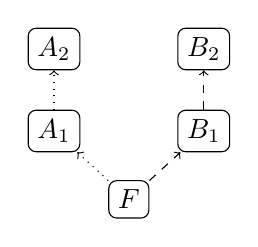
\begin{tikzpicture}[node distance=5mm,
      terminal/.style={rectangle,draw=black,rounded corners=1mm}]
\node (F) [terminal] {$F$};
\node (A1) [terminal,above left=of F] {$A_1$};
\node (A2) [terminal,above=of A1] {$A_2$};
\node (B1) [terminal,above right=of F] {$B_1$};
\node (B2) [terminal,above=of B1] {$B_2$};
\graph {
  (F) ->[dotted] (A1) ->[dotted] (A2);
  (F) ->[dashed] (B1) ->[dashed] (B2);
};
\end{tikzpicture}
\caption{Unslashed Progress Counterexample}\label{fig:unslashed-counterexample}
\end{figure}
The example is shown in Figure~\ref{fig:unslashed-counterexample}.
$F$ is the most recent finalized block, $A_1$ and $B_1$ immediate children of $F$,
and $A_2$ and $B_2$ immediate children (respectively) of $A_1$ and $A_2$.
Half of the validators have voted for the edges $F\!\!\rightarrow\!\! A_1$
and $A_1\!\! \rightarrow\!\! A_2$ (dotted arrows) and the other half of
the validators have voted for $F\!\! \rightarrow\!\! B_1$
and $B_1\!\! \rightarrow\!\! B_2$ (dashed arrows).
It is impossible to make a super-majority link from $F$ to any other block
without some validators being slashed.
A new edge from $F$ to a block one or two levels above $F$ would violate slashing
Condition I, because every validator already has votes with a target at that level.
An edge from $F$ to a block at any higher level would violate Condition II,
with the inner vote being that validator's vote for $A_1\!\! \rightarrow\!\! A_2$
or $B_1\!\! \rightarrow\!\! B_2$.

\section{Slashing Lower Bound}
\label{sec:bound}

When the set of validators is fixed, i.e. validators are not allowed to join or leave the network during the execution of the protocol, being a super-majority quorum depends only on the condition that the quorum's weight is at least $\frac{2}{3}$ of the total stake. Consequently, the intersection of two super-majority quorums in this setting must have at least $\frac{1}{3}$ of the total stake, and hence the lower bound of $\frac{1}{3}$ of the total stake being slashed in case of a violation of safety.

However, requiring that the set of validators be fixed is unrealistic, since the Beacon Chain protocol is a permissionless system, allowing nodes to join and leave (according to some activation and exit policies). Intuitively, nodes who have their deposits accepted may be activated at a block and remain active until they decide to leave or are forced to leave (when its deposited stake becomes too low due to repeated slashing for example), at which point the validator exits the active validator set. Having dynamic sets, however, means that, in case of a safety violation, we are less likely to be able to provably slash the misbehaving validators since they may now manage to ``escape'' before their deposits are actually slashed. Furthermore, active validator sets at two different branches of the block tree may be so much different that finding votes violating the conditions is a problem. The Beacon Chain protocol implements a set of elaborate activation and exit policies whose primary objective is to alleviate these potential problems (see~\cite{Beacon} for more details).

Our formalization of the protocol in Coq is guided by the level of abstraction given by Gasper~\cite{ButerinBHKPQRSWZ:2020}. As described in Section~\ref{sec:quorums}, the function \lstinline|vset| models the behavior of potentially changing validator sets by defining for each block a set of active validators. Recall the quorum intersection property \lstinline|q_intersection_slashed| that defines what it means to be ``slash-able'' in this context: there exists two super-majority quorums, with each quorum being a subset of a set of active validators of some block, such that their intersection is slashed (note how this property specializes to the $\frac{1}{3}$ bound if the set of validators is assumed fixed, i.e. when \lstinline|vset| is constant). Gasper expresses a lower bound on what can be provably slashed in this setting in terms of the churn of validator sets in the checkpoint block tree, which is practically useful as this churn can be controlled through validator activation and exit policies, effectively providing a mechanism to adjust the acceptable bound on what is guaranteed to be slashable.

To formalize this theorem, we first define activations and exits with respect to two validator sets.
\begin{lstlisting}
Definition activated (s1 s2: {set Validator}): {set Validator} :=
  s2 :\: s1.
Definition exited (s1 s2: {set Validator}): {set Validator} :=
  s1 :\: s2.
\end{lstlisting}
The symbol \lstinline|:\:| is for set difference. We also define activation and exit weights:
\begin{lstlisting}
Definition actwt (s1 s2: {set Validator}): nat :=
  wt (activated s1 s2).
Definition extwt (s1 s2: {set Validator}): nat :=
  wt (exited s1 s2).
\end{lstlisting}

We now have all the ingredients needed to formalize this theorem giving a lower bound on the amount of stake that can be provably slashed due to a violation:
\begin{lstlisting}
Theorem slashable_bound : forall st b0 b1 b2 b1_h b2_h k1 k2,
  k_finalized st b1 b1_h k1 ->
  k_finalized st b2 b2_h k2 ->
  b1 </~* b2 -> b2 </~* b1 ->
  exists (bL bR:Hash) (qL qR:{set Validator}),
    let v0 := vset.[vs_fun b0] in
    let vL := vset.[vs_fun bL] in
    let vR := vset.[vs_fun bR] in
    let aL := actwt v0 vL in
    let eL := extwt v0 vL in
    let aR := actwt v0 vR in
    let eR := extwt v0 vR in
    let xM := maxn (wt vL - aL - eR)  (wt vR - aR - eL) in
      qL \subset vL /\
      qR \subset vR /\
      wt (qL :&: qR) >= xM - one_third (wt vL) - one_third (wt vR).
\end{lstlisting}
The theorem states that if two conflicting blocks \lstinline|b1| and \lstinline|b2| are finalized, which is the premise of a safety violation, then we can find two quorums \lstinline|qL| (for some block \lstinline|bL|) and \lstinline|qR| (for some block \lstinline|bR|) such that the weight of the intersection \lstinline|(qL :&: qR)| is at least the quantity:
\begin{lstlisting}
  maxn (wt vL - aL - eR)  (wt vR - aR - eL) 
  - one_third (wt vL) 
  - one_third (wt vR)
\end{lstlisting}
where \lstinline|maxn| evaluates to the maximum of its two arguments. Note that this quantity is parameterized by the activation and exit weights (\lstinline|aL|,  \lstinline|aR|, \lstinline|eL| and \lstinline|eR|) with respect to a reference block \lstinline|b0|. The intersection of the two quorums is the set of validators that have violated the slashing conditions and are thus to be slashed. 

The proof follows the argument given in~\cite{ButerinBHKPQRSWZ:2020}, which is based on some basic properties of the \lstinline|wt| function (some of which were highlighted in Section~\ref{sec:validators} above). The proof also uses a number of basic set-theoretic lemmas and several inequalities on natural numbers from the Mathematical Components library, augmented with a few more lemmas in the files \lstinline|SetTheoryProps.v| and \lstinline|NatExt.v| in the project's repository. 

\section{Discussion}
\label{sec:discussion}

As we mentioned above, our strategy in developing the formalization in Coq is to have a model that matches as much as possible the level of abstraction of Gasper as described in~\cite{ButerinBHKPQRSWZ:2020}. The various representations in the model, e.g. the checkpoint block tree and validator sets and votes, along with the definitions and properties, such as those for justification, finalization and the theorem statements, are all based directly on the protocol's description. Nevertheless, one deviation from the description was made to avoid unnecessarily complicating the model. More specifically, our model uses the original Casper paper’s abstract treatment of checkpoint blocks~\cite{Buterin2017}, which does not explicitly use justified pairs as in Gasper~\cite{ButerinBHKPQRSWZ:2020}. Qualifying a justified block with the justification epoch is not needed in our model because it already abstracts blocks by their identifiers (hashes), which are assumed unique. So even if the same block is justified for two different epochs, the model already treats these two justification instances as two distinct blocks. The additional information that the two instances actually point to the same block is irrelevant to the model.

Furthermore, the formalization is naturally much more rigorous than a high-level description and makes explicit all the assumptions needed for the arguments to hold. We highlight below some of the important assumptions that the model explicitly specifies for the plausible liveness property:
\begin{itemize}
\item Supermajority quorums are non-empty (\lstinline|quorum_2_nonempty|), which implies the weaker condition that validator sets are non-empty. No progress can be made with an empty quorum (or validator set).
\item Justification links must be proper: In addition to being a supermajority link, a justification link must be a valid forward link in the block tree with the target's height being greater than the source’s.
\item Only the votes that originate from the validator set of the target block being voted for are considered (\lstinline|votes_from_target_vset|). This also implies Justification is preserved when the state is expanded with new votes (coming from validators in the validator set of the justified block). Although this is not explicitly stated in Gasper, the Beacon Chain protocol's implementation already ignores votes that do not satisfy this assumption.
\item For any block, all validators of a supermajority set of that block produce only good votes: votes that have justified sources and that represent valid forward links in the block tree (\lstinline|good_votes|). Votes with unjustified sources or ones that do not represent proper forward links in the checkpoint tree do not violate any slashing conditions themselves, but can prevent a validator from contributing to progress, because votes spanning over such bad votes would violate slashing condition II. This is also checked for in the implementation of the protocol.
\item For any block, there exists a supermajority whose validators have not been slashed (\lstinline|two_thirds_good|). Progress is meaningful only if it can be made by validators following the protocol.
%These are in addition to assumptions given explicitly in the paper, like the assumption that the underlying block-producing protocol continues to generate new blocks that are sufficiently high in the tree (In the model, blocks exist sufficiently high over the highest justified block -- defined by \lstinline|blocks_exist_high_over|).
\end{itemize}

Finally, going through this exercise of modeling and verification helps in refining the definitions and arguments of Gasper. For instance, the Coq model does not assume that the genesis block is finalized, but it can be proved that this property follows from the model, under certain good-behavior assumptions that we already make for safety and liveness. This suggests a possible simplification to the definition of finalization, provided that these assumptions are given clearly. Another example is the formalization of the slashable bound theorem, which suggested improvements to the statement and argument of the theorem in Gasper's description and eventually the description was updated to incorporate them. In particular, the assumption that the reference block \lstinline|B0| is finalized was shown unnecessary, and in fact this block can potentially be any block in the block tree. Furthermore, the statement of the theorem and how its argument uses Lemma 8.3 were made more accurate, matching the formalization in the model.


\section{Conclusion}
\label{sec:conclusion}

We presented a formalization of the finality mechanism of Gasper (most up-to-date Casper version) in Coq, along with proofs of three major properties: accountable safety, plausible liveness and the slashing lower bound, all in one model supporting the general dynamic validator sets setting. 
These proofs clarified the assumptions needed for the properties stated in
the Gasper paper~\cite{ButerinBHKPQRSWZ:2020}, and helped further improve its theorem statements and arguments.
Our formalization work paves the way for proving accountable safety, 
plausible liveness and the slashable bound for the state-transition function of the Beacon Chain protocol's
implementation~\cite{Beacon}.

%Our goal is to have our Coq implementation correspond as closely as
%possible with the implementation in~\cite{Beacon}. This gives us the greatest
%assurance that our proven properties hold in the most up-to-date Casper version.

%\begin{lstlisting}[language=Coq]
%Definition fork (bc1 bc2 : seq T) :=
% ~ (is_prefix bc1 bc2 \/ is_prefix bc2 bc1).
%\end{lstlisting}

%\section{Discussion}

%% Acknowledgments
\begin{acks}

We thank Danny Ryan, Carl Beekhuizen, Martin Lundfall, Yan Zhang and Aditya Asgaonkar from the Ethereum Foundation for their valuable feedback and comments. This work was funded by the Ethereum Foundation.
  
%                                        %% contents suppressed with 'anonymous'
%  %% Commands \grantsponsor{<sponsorID>}{<name>}{<url>} and
%  %% \grantnum[<url>]{<sponsorID>}{<number>} should be used to
%  %% acknowledge financial support and will be used by metadata
%  %% extraction tools.
%  This material is based upon work supported by the
%  \grantsponsor{GS100000001}{National Science
%    Foundation}{http://dx.doi.org/10.13039/100000001} under Grant
%  No.~\grantnum{GS100000001}{nnnnnnn} and Grant
%  No.~\grantnum{GS100000001}{mmmmmmm}.  Any opinions, findings, and
%  conclusions or recommendations expressed in this material are those
%  of the author and do not necessarily reflect the views of the
%  National Science Foundation.
\end{acks}


%% Bibliography
\bibliography{bib}


%% Appendix
%\appendix
%\section{Appendix}
%
%Text of appendix \ldots

\end{document}
